\documentclass[a4paper]{scrartcl}

% Font and Language
\usepackage[utf8]{inputenc}
\usepackage[english]{babel}
\usepackage[rm,light]{roboto}
\usepackage{hyperref}
\usepackage{xurl}
\usepackage{cleveref}
\KOMAoptions{fontsize=11pt}

\usepackage{tikz}
\usetikzlibrary{	
	fit,
	arrows,
	positioning	
}

\tikzset{
%Define standard arrow tip
>=stealth',
%Define style for boxes
punkt/.style={
	rectangle,
	rounded corners,
	draw=black, very thick,
	text width=6.5em,
	minimum height=2em,
	text centered},
%Define style for placeholder boxes
placeholder/.style={
	rectangle,
	rounded corners,
	draw=white, very thick, opacity=0.0,
	text width=6.5em,
	minimum height=2em,
	text centered},
% Define arrow style
pil/.style={
	->,
	thick,
	shorten <=2pt,
	shorten >=2pt,},
lip/.style={
	<-,
	thick,
	shorten <=2pt,
	shorten >=2pt,},
lil/.style={
	<->,
	thick,
	shorten <=2pt,
	shorten >=2pt,}
}
% Set Metadata
\title{FOSS implementation of the WorkAdventure Admin Services}
\author{Tobias Tefke $<$t.tefke@stud.fh-sm.de$>$}

% Paragraphs: on = vertical skip ; off = horizontal skip
\KOMAoptions{parskip=on}
\begin{document}
	\maketitle
	\section{Introduction}
	\enlargethispage{\baselineskip}
	\enlargethispage{\baselineskip}
	Workadventure\footnote{\url{https://workadventu.re} (acc. 09/19/2021)} is a web application which features online meetings.
	It differs from other online conferencing solutions by its design.
	The applications resembles a game in eight bit optics.
	Participants have avatars which can move on a two-dimensional map. 
	If characters get close to each other they can talk to each other.
	The talk can be left by moving away.
	Furthermore, it is possible to embed special actions on the map tiles.
	This includes opening websites and starting Jitsi conferences\footnote{\url{https://workadventu.re/map-building/opening-a-website.md} and \url{https://workadventu.re/map-building/meeting-rooms.md} (acc. 09/19/2021)}.
	\section{Motivation}
	An open source version of WorkAdventure can be self-hosted\footnote{\url{https://github.com/thecodingmachine/workadventure} (acc. 09/19/2021)}.
	However, a paid version with additional features is available.
	These features include sending global messages and access control.
	If someone decides to use these functions, a proprietary administration component has to be included.
	Furthermore, a fee based on the number of simultaneous connections must be paid\footnote{\url{https://workadventu.re/pricing} (acc. 09/19/2021)}.
	Moreover, user-specific data is being exchanged with the administration component.
	This makes it hard to integrate WorkAdventure into environments in which user data must be well protected, e.g. education institutions.
	In order to mitigate the mentioned problems, it was decided to re-implement the administration services as open-source software.
	\section{Background}
	\enlargethispage{\baselineskip}
	\enlargethispage{\baselineskip}
	The communication messages sent between the proprietary and open-source service are defined in the pusher and back-components\footnote{\label{communication-messages}\url{https://github.com/thecodingmachine/workadventure/blob/develop/pusher/src/Services/AdminApi.ts} and \url{https://github.com/thecodingmachine/workadventure/blob/develop/back/src/Services/AdminApi.ts} (acc. 09/19/2021)}.
	The open source components request services from the admin services by sending HTTP requests using axios\footref{communication-messages}\footnote{\url{https://www.npmjs.com/package/axios} (acc. 09/19/2021)}. Here, the WorkAdventure services have to authenticate by sending an authentication token\footref{communication-messages}.
	If the authentication succeeds, the admin API responds with a JavaScript object containing the requested information, serialized in JSON\footref{communication-messages}.
	\section{Implementation}
	Using the knowledge about how communication works, it is possible to reimplement the proprietary services. A coarse overview about the reimplementation is shown in \Cref{structural_overview}. The HTTP requests are sent to the URL of the admin services. This URL is set to our admin service implementation. There, an nginx server handles the requests and  the requested PHP scripts are being called. PHP reads the necessary data to respond from an SQL database and returns the expected answer encoded in JSON. The encoded data is then being returned to WorkAdventure, where it can be further processed.\\
	Furthermore, a Website is being hosted on the nginx server, making it possible for the administrator to perform CRUD operations on the information stored in the database using a graphical user interface.
	\begin{figure}[htb]
		\centering
		\resizebox{\textwidth}{!}{%
			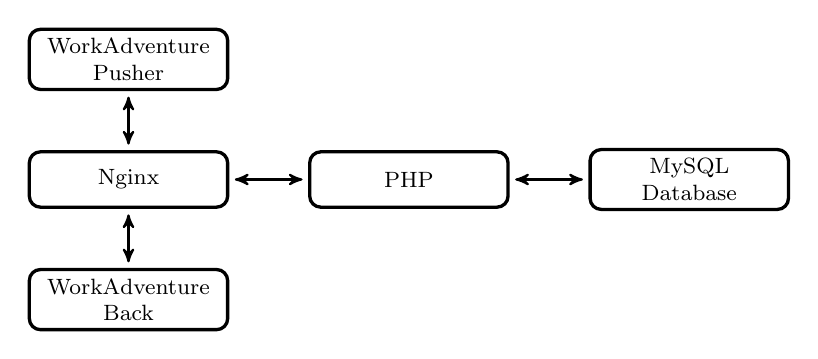
\begin{tikzpicture}[auto]
				\tikzstyle{every node}=[font=\footnotesize]
				\node[punkt] (sql) {MySQL Database};
				\node[punkt, left=1cm of sql] (php) {PHP} edge[lil] (sql);
				\node[punkt, left=1cm of php] (nginx) {Nginx} edge[lil] (php);
				\node[punkt, left=1cm of nginx,above=0.75cm of nginx] (pusher) {WorkAdventure Pusher} edge[lil] (nginx);
				\node[punkt, left=1cm of nginx,below=0.75cm of nginx] (back) {WorkAdventure Back} edge[lil] (nginx);
			\end{tikzpicture}
		}
		\caption{Structural overview about how the administrative components interact with each other.}
		\label{structural_overview}
	\end{figure}
\end{document}